\documentclass{article}

\usepackage[dblblindworkshop]{neurips_2026}
\workshoptitle{Representations for the Physical Sciences Workshop}

\usepackage[utf8]{inputenc}
\usepackage[T1]{fontenc}
\usepackage[bookmarks=false]{hyperref}
\usepackage{url}
\usepackage{booktabs}
\usepackage{amsfonts}
\usepackage{amsmath}
\usepackage{nicefrac}
\usepackage{microtype}
\usepackage{graphicx}
\usepackage{xcolor}

\title{Learning Conway's Game of Life with CNN-Transformer Hybrids:\\
Architecture Scaling, Exposure Bias, and Activation Inductive Bias}

\author{%
  Anonymous Author(s) \\
  Affiliation \\
  Address \\
  \texttt{email}
}

\begin{document}

\maketitle

\begin{abstract}
We study how a CNN-Transformer hybrid learns the one-step transition rule
of Conway's Game of Life (GoL) on a $40\times40$ toroidal grid. Starting
from a model trained with pure teacher forcing, we show that
autoregressive rollout suffers from exposure bias, that a
straight-through-estimator (STE) multi-step scheme fails due to a
systematic gradient bias, and that scheduled sampling resolves this
cleanly. We further show that once a model saturates its capacity,
scaling the training set five-fold \emph{regresses} tail-case accuracy in
a way invisible to aggregate validation metrics, while scaling the model
five-fold instead eliminates essentially all remaining errors. Motivated
by recent work on activation-function inductive bias for cellular
automata, we independently reproduce the finding that a learnable
second-degree polynomial activation lets a 25--34 parameter CNN learn GoL
reliably where ReLU fails, and report a negative result transferring this
activation to our larger multi-step model. Finally, we measure how much
patch embeddings change under rotation, reflection, and translation for
two models of different capacity (V8, V10), finding that both are nearly
invariant on a sparse glider but that our larger model is roughly twice
as sensitive as the smaller one on dense random grids, across every
transform tested.
\end{abstract}

\section{Problem and architecture}
\label{sec:arch}

GoL is a deterministic cellular automaton: each cell's next state depends
only on its own state and its 8-neighbor live count (B3/S23). We treat one
GoL step as image-to-image prediction on a periodic $40\times40$ grid. Our
core architecture is a CNN-Transformer hybrid: two circular-padded
convolutions extract local, translation-equivariant features respecting
the torus topology; these are cut into non-overlapping $4\times4$ patches,
linearly projected, combined with a \emph{learned} absolute positional
embedding, passed through a Transformer encoder for global mixing, and
projected back to per-cell logits. GoL is a natural stress test for
learned representations: prior work shows plain feed-forward networks
struggle to learn it reliably at all \citep{springer2021minimal}, and the
Transformer stage \citep{vaswani2017attention} trades the CNN's clean
equivariance guarantee for long-range context (Section~\ref{sec:embed}).
This V4 design is itself the fourth step of an earlier architecture
search, each step fixing one identified issue: V1 (avg-pooled tokens,
learned positional embedding, zero-padding) $\to$ V2 (swaps in a
\emph{fixed sinusoidal} positional embedding to remove a right-edge
rollout artifact) $\to$ V3 (swaps avg-pooling for a lossless
flatten-and-project tokenization, reverting to a learned embedding)
$\to$ V4 (swaps zero-padding for circular padding, fixing incorrect
boundary neighbor counts). V5 onward (Section~\ref{sec:evolution}) all
train this same V4 architecture under different regimes and sizes.

\section{Training evolution: two failure modes and their fixes}
\label{sec:evolution}

\paragraph{Exposure bias.} A model trained with pure single-step teacher
forcing (V5) scores $>99\%$ precision/recall on held-out single steps but
collapses under autoregressive rollout, since it never sees its own
(imperfect) outputs during training. A straight-through-estimator (STE)
multi-step scheme intended to fix this instead \textbf{diverges} after
epoch 5, which we trace to a systematic gradient bias from the STE's hard
threshold. Replacing STE with \emph{scheduled sampling}
\citep{bengio2015scheduled} --- gradually increasing the probability of
feeding the model its own previous prediction --- fixes this cleanly and
stably (V7).

\paragraph{A hidden data-scaling regression.} Upsampling high-density
configurations $3\times$ (V8) improves per-grid accuracy further (291K
params). Naively scaling the \emph{training set} $5\times$ (V9) leaves
aggregate validation metrics statistically unchanged, but a density-
stratified failure search (500 grids at each of five densities, fixed seed
across models) reveals V9's error count at density 0.80 is nearly
\textbf{seven times worse} than V8's (22{,}190 vs.\ 3{,}358 summed
false positives/negatives) --- invisible in aggregate metrics alone.
Instead of more data, we scale the \emph{model}: V10 (5.15$\times$ V8's
size, $1.5$M params, trained from scratch) achieves \textbf{zero errors}
across all 2{,}500 test grids at every density (Table~\ref{tab:summary},
Figure~\ref{fig:v10}). The lesson: once capacity saturates, more data can
silently trade average-case for tail-case performance, detectable only by
per-subgroup error auditing, not validation loss.

\begin{table}[t]
\centering
\small
\resizebox{\linewidth}{!}{%
\begin{tabular}{lp{4.3cm}ccl}
\toprule
Ver.\ & Key change & Val.\ loss & Prec./Rec.\ & Status \\
\midrule
V1 & Baseline: avg-pool tokens, learned PE, zero-pad & ---\textsuperscript{b} & --- & Edge artifacts; rollout freezes to a blob \\
V2 & Learned PE $\to$ fixed sinusoidal PE & ---\textsuperscript{b} & --- & Unstable training; no rollout improvement \\
V3 & Avg-pool $\to$ flatten+linear tokenization & 0.021 & --- & \textbf{Fixes} avg-pool bottleneck; first realistic rollouts \\
V4 & Zero-padding $\to$ circular padding & 0.226 & 100\% / 94.3\% & Fixes boundary bug; base arch.\ for V5+ \\
\addlinespace
V5 & Single-step teacher forcing & 0.201 & 99.4\% / 99.7\% & Collapses under rollout \\
V6 & +STE multi-step & 0.234\textsuperscript{a} & 92.7\% / --- & \textbf{Diverges} \\
V7 & STE $\to$ scheduled sampling & 0.201 & 99.7\% / 100\% & Stable \\
V8 & +3$\times$ high-density upsample & 0.201 & 100\% / 99.9\% & Best per-grid (291K params) \\
V9 & +5$\times$ all data & 0.201 & 99.7\% / 99.6\% & \textbf{Regressed} tail errors \\
V10 & 5.15$\times$ model size & 0.199 & 100\% / 100\% & \textbf{Zero errors}, 2{,}500/2{,}500 \\
\bottomrule
\end{tabular}%
}
\caption{Version summary, spanning the V1--V4 architecture search
(Section~\ref{sec:arch}) and the V5--V10 training-regime
search (Section~\ref{sec:evolution}). \textsuperscript{a}V6's best epoch
before divergence. \textsuperscript{b}V1/V2 reported only aggregate val
accuracy (89.4\% and 84\% respectively), not loss or a precision/recall
split.}
\label{tab:summary}
\end{table}

\begin{figure}[t]
\centering
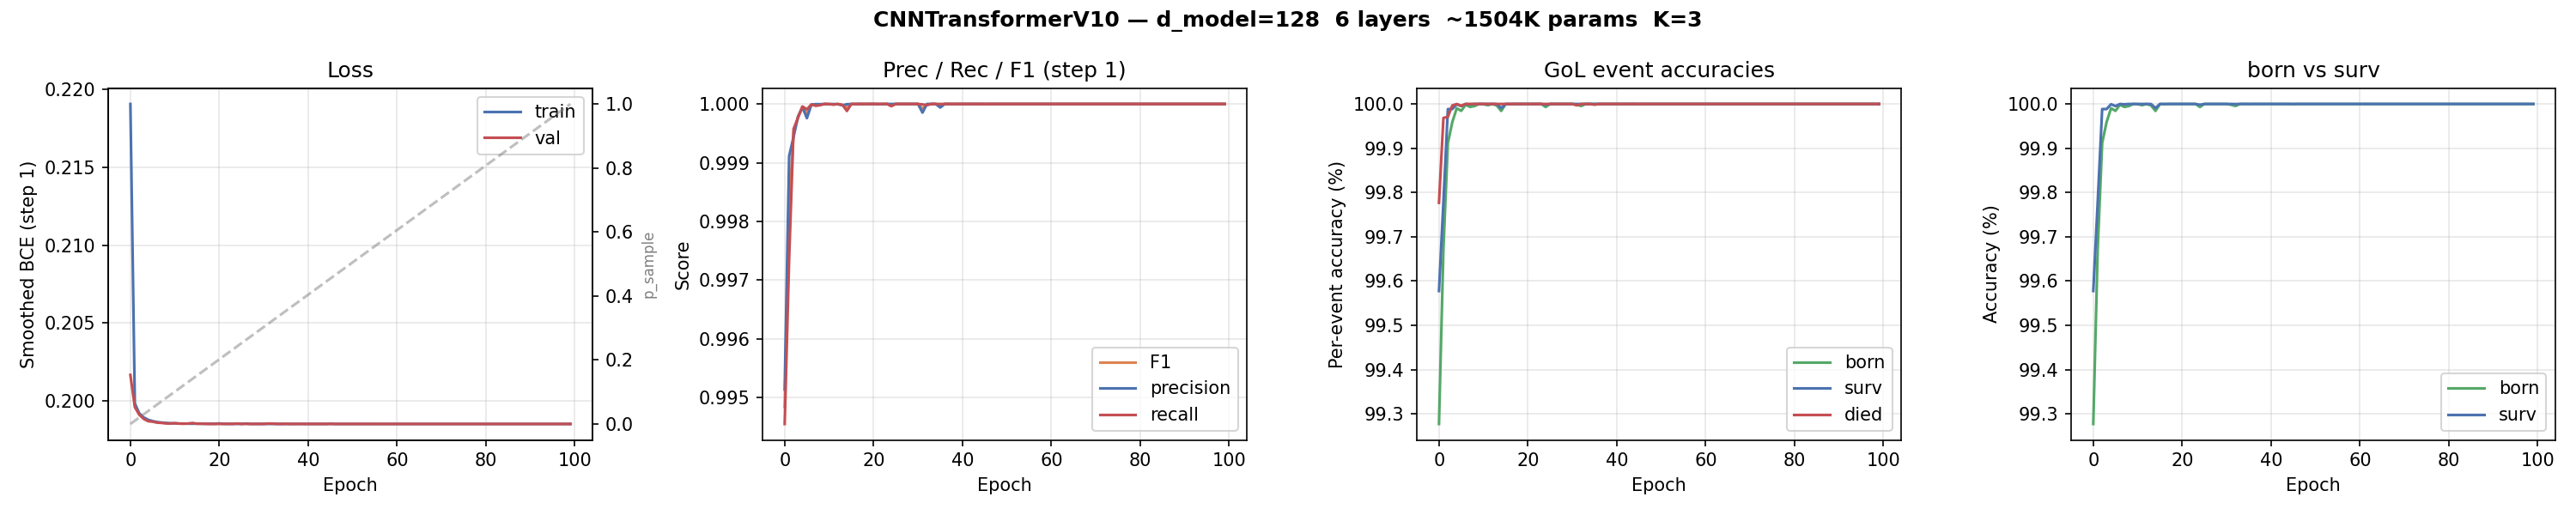
\includegraphics[width=0.85\linewidth]{figures/v10_loss.png}\\[0.5em]
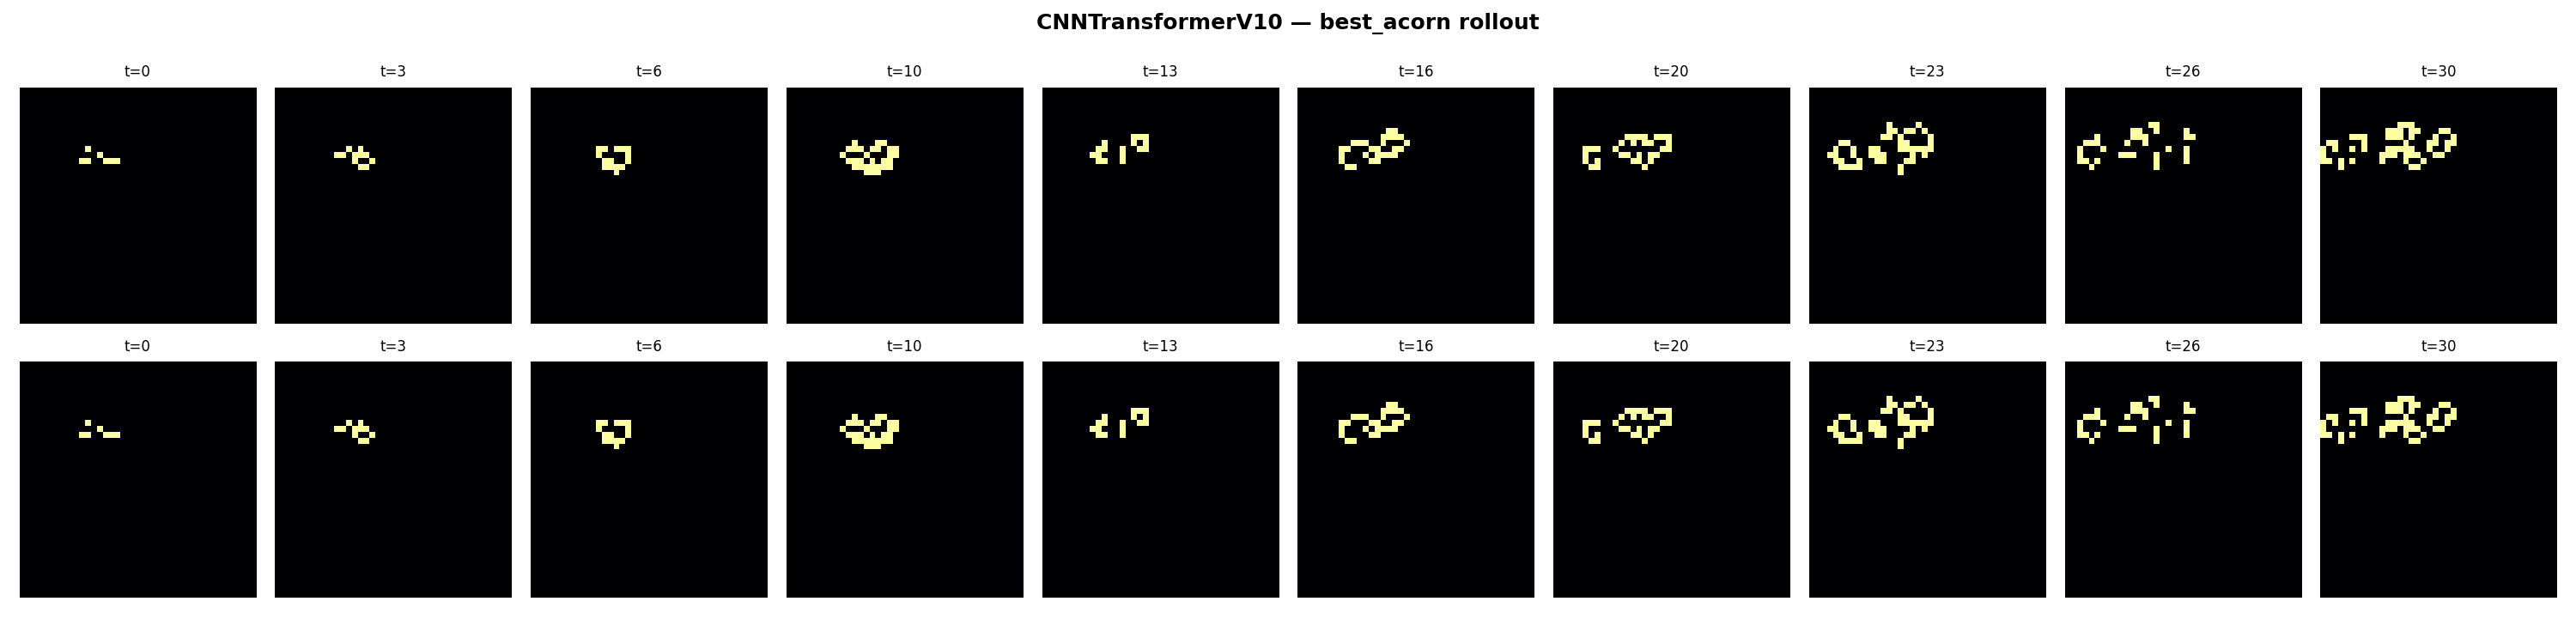
\includegraphics[width=\linewidth]{figures/v10_rollout_acorn.png}
\caption{Top: V10 training curve. Bottom: a 30-step autoregressive
rollout of the \emph{acorn} methuselah --- a 7-cell seed that grows into
a large, long-lived chaotic pattern --- true trajectory (top row) vs.\
V10's autoregressive prediction (bottom row); V10 tracks the true
trajectory exactly at every shown step, and makes zero errors across
2{,}500 held-out grids overall.}
\label{fig:v10}
\end{figure}

\section{Embedding geometry: does model capacity affect equivariance?}
\label{sec:embed}

A CNN feature map is a \emph{physical} embedding: convolution's
translation-equivariance means shifting the input shifts the feature map
identically. A Transformer's patch embeddings, after a learned absolute
positional embedding, have no such guarantee --- each position slot is an
independently learned vector unrelated to its neighbors, and nothing in
the architecture guarantees invariance under rotation or reflection
either. We measure this directly for two stable, well-converged models of
different capacity, V8 (291K params) and V10 (1.5M params), on two base
patterns --- a sparse glider and a dense random grid (density $0.5$) ---
under nine individual transforms each: translation by 4 cells in each of
the four cardinal directions, rotation by $90^\circ/180^\circ/270^\circ$,
and horizontal/vertical reflection. For each of the 18 (pattern, transform)
cases we measure post-Transformer cosine similarity between the original
grid's embedding and the transformed grid's embedding; higher similarity
means the embedding changed less under that specific transform.

Breaking this down by individual case (four translation directions,
three rotation angles, two reflection axes) and by pattern type reveals
that pattern sparsity, not transform type, is what actually matters
(Figure~\ref{fig:pe-verify}, top). For the sparse \emph{glider}, both
models are close to fully invariant to every transform ($0.97$--$0.99$
similarity, V8 and V10 alike) --- unsurprising, since a glider occupies
only 3 of 100 patches and most patches are unchanged background under
any of these transforms. For the dense \emph{random} grid, the two
models diverge sharply: V8 stays around $0.79$--$0.81$ across all nine
cases, while V10 drops to $0.42$--$0.47$ --- roughly half. As in
Section~\ref{sec:evolution}, sparse and dense configurations behave
completely differently, and an evaluation limited to sparse patterns
(where both models look equally equivariant) would have entirely missed
V10's much larger sensitivity on dense grids. This is consistent with
V10 having learned more content-sensitive, less redundant embeddings
overall as a side effect of reaching much higher task accuracy
(Section~\ref{sec:evolution}), rather than the larger model specifically
losing geometric structure.

This measurement also suggests a concrete direction for future work:
since GoL's transition rule is itself translation- and rotation-invariant,
a model whose representations shared that invariance would have less to
learn from data alone. Building on the diagnostic here, one could train
with an explicit consistency loss between a grid's embedding and its
transformed counterpart's, or design the positional encoding and
attention mechanism to be equivariant by construction, and use the same
per-case measurement to check whether the resulting model both matches
this invariance and retains V10's dense-grid accuracy.

\section{Independent verification: polynomial activations for GoL}

Motivated by a recent claim that a learnable second-degree polynomial
activation $\phi(x) = w_0 + w_1 x + w_2 x^2$ lets a minimal CNN learn GoL
reliably where ReLU fails almost completely \citep{ahmed2026polynomial},
we independently reproduced this rather than taking it on faith. We built
two CNNs matching the paper's minimal architecture (two $1{\times}1$
convolutions plus one $3{\times}3$ circular-padded convolution),
\textbf{identical except for the activation function}, matching the
paper's reported parameter counts exactly (ReLU: 25 params, polynomial:
34 params). Trained single-step, teacher-forcing, over 10 random seeds:
ReLU converges to perfect validation accuracy in only $1/10$ seeds (mean
final accuracy $89.4\%$), while the polynomial activation converges in
$10/10$ seeds ($100.0\%$ mean accuracy), confirming the claim on our own
toroidal GoL setup (Figure~\ref{fig:pe-verify}, bottom). We then
attempted to transfer this activation into our larger multi-step model
(same size as V8) by replacing GELU with polynomial activations in the
CNN stage; this \textbf{failed}, diverging sharply after epoch 5 under
scheduled sampling, likely because the unbounded $w_2 x^2$ term compounds
through the autoregressive feedback loop in a way it cannot in a
single-step setting. Candidate fixes (a bounded/saturating variant, a
separate learning rate for polynomial coefficients) were identified but
not yet pursued.

\begin{figure}[t]
\centering
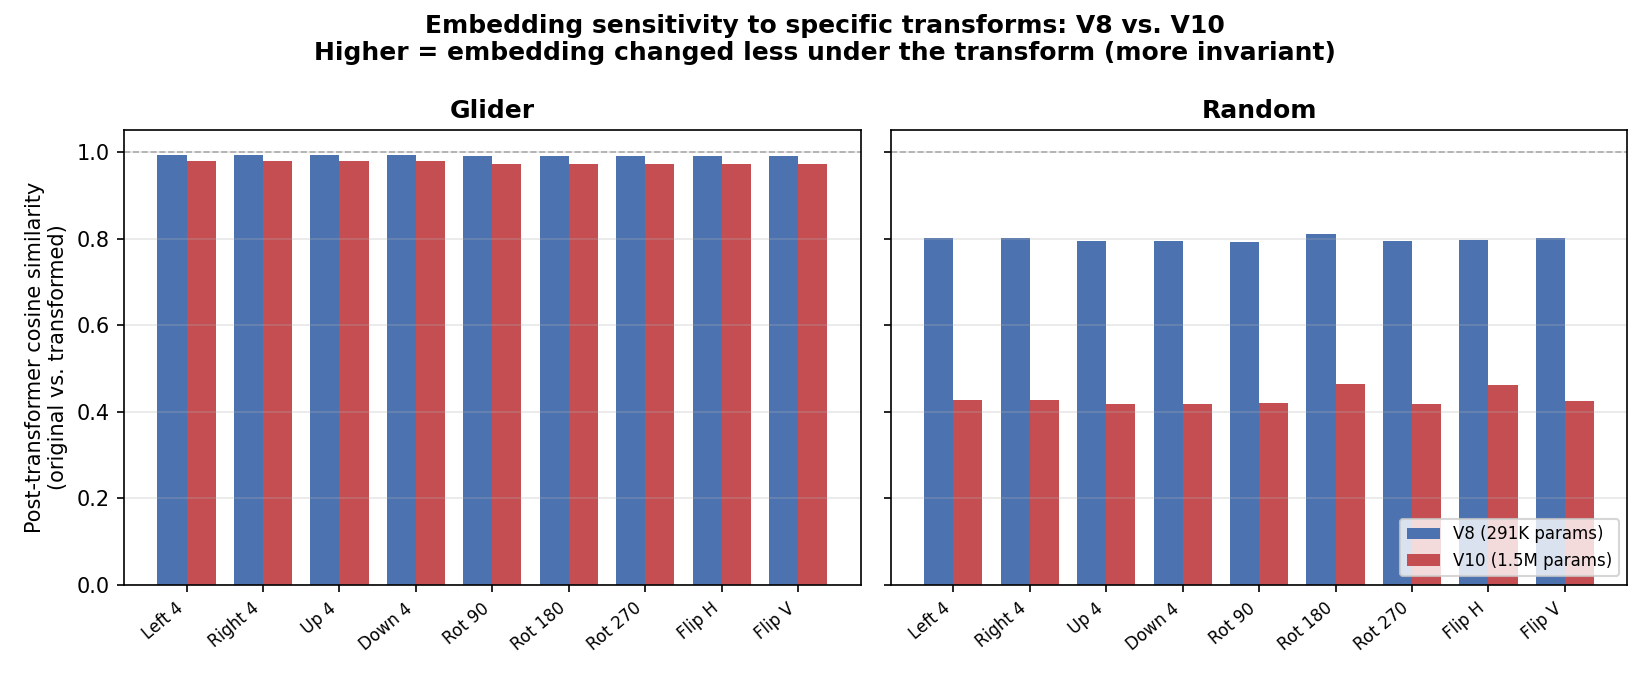
\includegraphics[width=\linewidth]{figures/v8_v10_transform_equivariance_detailed.png}\\[0.5em]
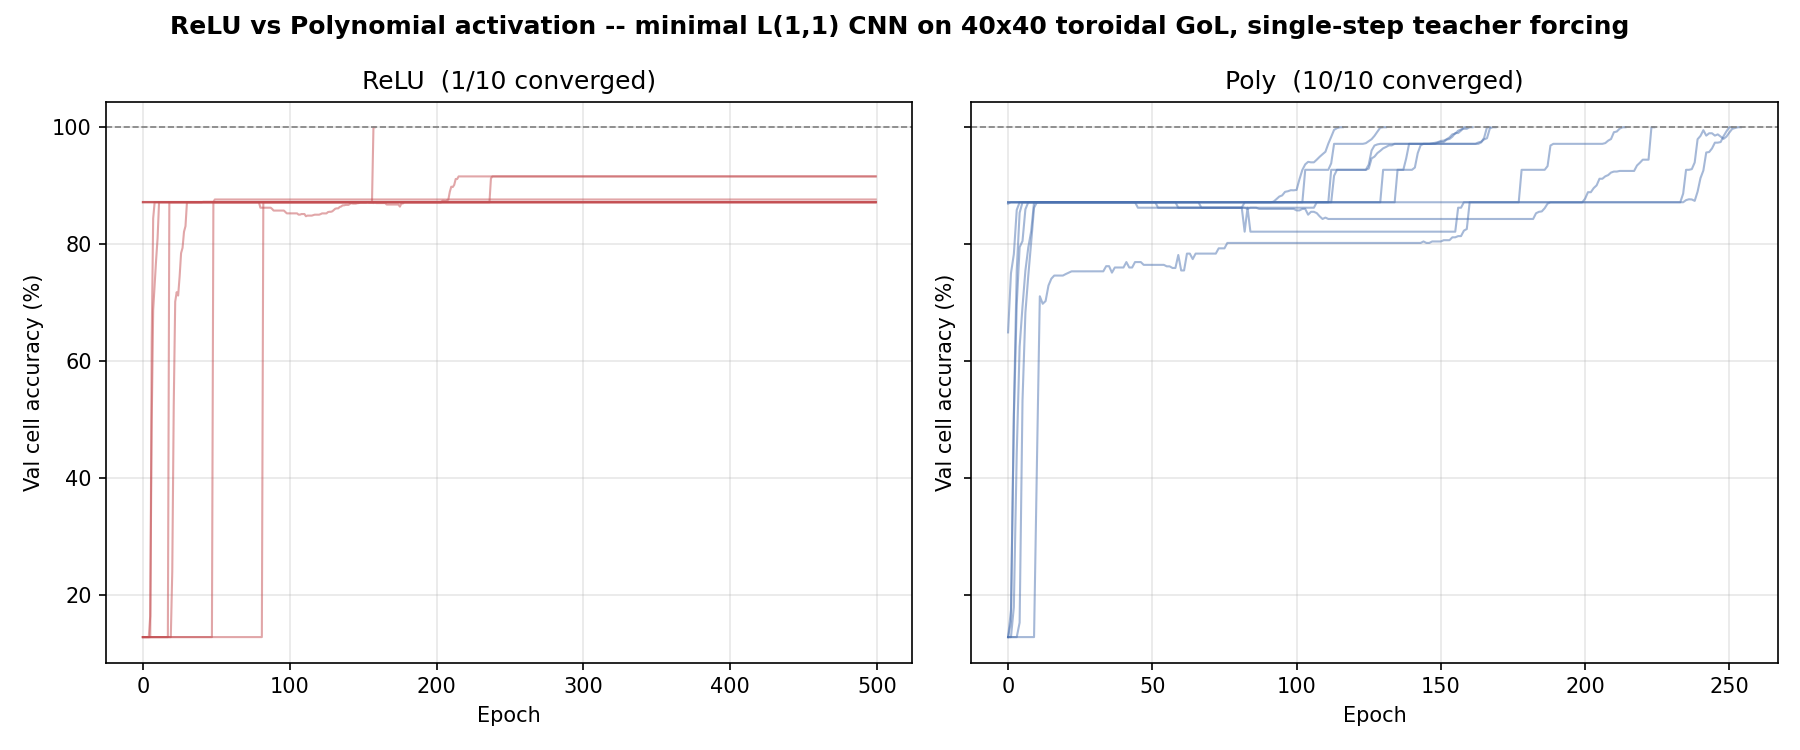
\includegraphics[width=0.75\linewidth]{figures/relu_vs_poly_convergence.png}
\caption{Top: post-Transformer embedding cosine similarity for each of
9 individual transforms (4 translation directions, 3 rotations, 2
reflections), separately for a sparse glider and a dense random grid,
V8 vs.\ V10; higher means the embedding changed less under that
transform. Bottom: validation accuracy over training, 10 seeds per
activation, on a minimal 25/34-parameter CNN; polynomial activation
converges reliably where ReLU does not.}
\label{fig:pe-verify}
\end{figure}

\section{Conclusion}

Three practical lessons emerge. First, autoregressive exposure bias is
best fixed with scheduled sampling rather than a hard differentiable
relaxation (STE), which can introduce its own destabilizing gradient
bias. Second, aggregate validation metrics can hide severe, density-
specific regressions; per-subgroup error auditing is necessary once a
model is scaled with more data rather than more capacity. Third, an
activation function's inductive-bias advantage demonstrated at minimal
scale and single-step training does not automatically transfer to a
larger, multi-step, autoregressively-trained model --- the interaction
between an activation's stability properties and the training regime
matters as much as the activation itself.

\bibliographystyle{plainnat}
\bibliography{references}

\end{document}
